\documentclass[11pt]{article}
\usepackage[utf8]{inputenc}
\usepackage[letterpaper, margin=0.75in]{geometry}
\usepackage{amsmath}
\usepackage{amssymb}
\usepackage{amsfonts}
\usepackage{enumitem}
\usepackage{chemfig}
\usepackage{tikz}
\usepackage{graphicx}

\setlength{\parindent}{0pt}
\setlength{\parskip}{1em}

\newcommand{\headerbox}{
    \noindent\begin{tabular}{|p{11cm}|p{5.5cm}|}
    \hline
    \scriptsize \textbf{Communication:} & \scriptsize \textbf{Overall:}\\
    \scriptsize Language: easy to understand, answers question, follows instructions, concise, precise & \\
    \scriptsize Chemistry: proper vocab, notation, spacing, logical & \scriptsize \space\space \space\space vague/basic/OK/good/clearly written \\
    \scriptsize Math: organized, units, sig digs, math notation, concluding statement, spacing & \\
    \hline
    \end{tabular}
    \vspace{1em}
}

\begin{document}

\headerbox

\vspace{0.2cm}
SCH4U \hfill Name: \underline{\hspace{5cm}} \\
\indent \hfill Monday, March 1, 2025

\begin{center}
    \Large \textbf{Unit 1: Structures \& Properties Test}
\end{center}

\begin{center}
\begin{tabular}{|lc|lc|}
\hline
Total: & /35 & Comm: & /10 \\
\hline
\end{tabular}
\end{center}

\begin{enumerate}
    \item {[2 marks]} What is wrong with the following Bohr-Rutherford diagram with regards to Quantum Mechanics? Be specific.
    
    \begin{minipage}{0.3\textwidth}
        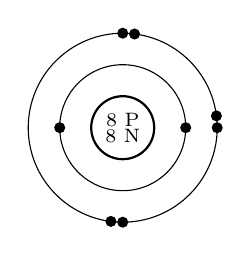
\begin{tikzpicture}
            \draw[thick] (0,0) circle (0.4cm);
            \node at (0,0.1) {\scriptsize 8 P};
            \node at (0,-0.1) {\scriptsize 8 N};
            \draw (0,0) circle (0.8cm);
            \draw (0,0) circle (1.2cm);
            % Electrons
            \fill (0.8,0) circle (2pt);
            \fill (-0.8,0) circle (2pt);
            \fill (0,1.2) circle (2pt);
            \fill (0.15,1.19) circle (2pt);
            \fill (0,-1.2) circle (2pt);
            \fill (-0.15,-1.19) circle (2pt);
            \fill (1.2,0) circle (2pt);
            \fill (1.19,0.15) circle (2pt);
        \end{tikzpicture}
    \end{minipage}
    \begin{minipage}{0.65\textwidth}
        \vspace{3cm}
        \hrulefill
        
        \hrulefill
    \end{minipage}

    \item {[3 marks]} Below is the emission spectra for hydrogen when an electron falls to $n = 2$. Where would an emission line for hydrogen be if an electron falls from $n = 5$ to $n = 3$? Indicate the location of this new emission line relative to the other emission lines. Is this energy transition high energy or low energy? Explain with or without a diagram. Calculations are not needed to answer this question.

    \begin{center}
    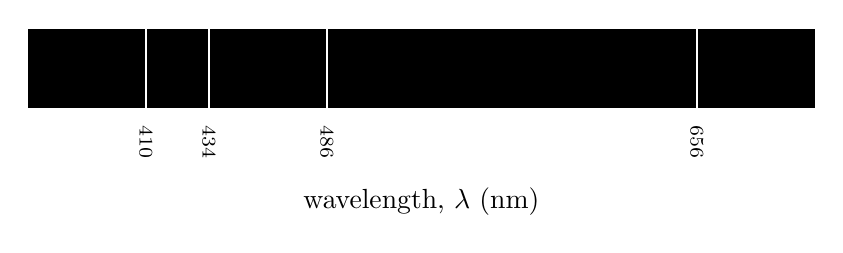
\begin{tikzpicture}
        % The black spectral bar
        \fill[black] (0,0) rectangle (10, 1);
        
        % Emission lines (white) and wavelength labels (black, below)
        
        % 410 nm
        \draw[white, thick] (1.5, 0) -- (1.5, 1);
        \node[black, rotate=-90, anchor=west] at (1.5, -0.1) {\scriptsize 410};
        
        % 434 nm
        \draw[white, thick] (2.3, 0) -- (2.3, 1);
        \node[black, rotate=-90, anchor=west] at (2.3, -0.1) {\scriptsize 434};
        
        % 486 nm
        \draw[white, thick] (3.8, 0) -- (3.8, 1);
        \node[black, rotate=-90, anchor=west] at (3.8, -0.1) {\scriptsize 486};
        
        % 656 nm
        \draw[white, thick] (8.5, 0) -- (8.5, 1);
        \node[black, rotate=-90, anchor=west] at (8.5, -0.1) {\scriptsize 656};
        
        % Axis label
        \node[black] at (5, -1.2) {wavelength, $\lambda$ (nm)};
    \end{tikzpicture}
    \end{center}
    \vspace{3cm}
\end{enumerate}

\newpage
\vspace*{0pt}
\headerbox

\begin{enumerate}[resume]
    \item {[6 marks]} Assuming there is enough energy to do so, write out the full/longhand electron configuration for the most stable form of Ru, $\text{Ru}^{3+}$ \& $\text{Ru}^{6+}$. Rank the three electron configurations in order of stability ($1 = \text{most stable}$). Ru is element 44.
    \vspace{5cm}

    \item {[2 marks]} Is the most stable electron configuration for an atom or ion always anomalous? Explain \& provide an example to support your answer.
    \vspace{4cm}

    \item {[4 marks]} Predict two realistic ionic charges for F$\ell$ (element 114). Write the shorthand electron configuration only. Justify your answer.
    \vspace{5cm}
\end{enumerate}

\newpage
\vspace*{0pt}
\headerbox

\begin{enumerate}[resume]
    \item {[3 marks]} Draw the ELD (energy level diagram) for neutral ground state As (element 33). Label the subshells.
    
    \vspace{5cm}

    \item {[3 marks]} Draw the most stable Lewis structure of $\text{XeF}_4^{2+}$. Verify your answer using formal charges.
    \vspace{4cm}

    \item {[2 marks]} Why is anomalous electron configuration not the same as hybridization? Provide an example.
    \vspace{4cm}

    \item {[4 marks]} Draw the orbital overlap showing the bonding in the following structure. Use different colours for each bond (if you have them). Label each bond as being $\sigma$ or $\pi$.
    
    \space\space\space \chemfig{H-Si(-[6]F)=O}
    \vspace{5cm}
\end{enumerate}

\newpage
\vspace*{0pt}
\headerbox

\begin{enumerate}[resume]
    \item {[2 marks]} What is the same \& what is different between the following: $\text{AB}_2\text{E}$ \& $\text{AB}_2\text{E}_2$? Be precise.
    \vspace{4cm}

    \item {[2 marks]} Why are ionic solids brittle? What is unique about the structure that allows it to do so? Provide an example of an ionic solid.
    \vspace{3cm}

    \item {[2 marks]} Explain the humour behind the meme. Be sure to explain/describe the theory needed in order to fully appreciate the chemistry humour in the meme.
    
        \begin{minipage}{0.4\textwidth}
            \centering
            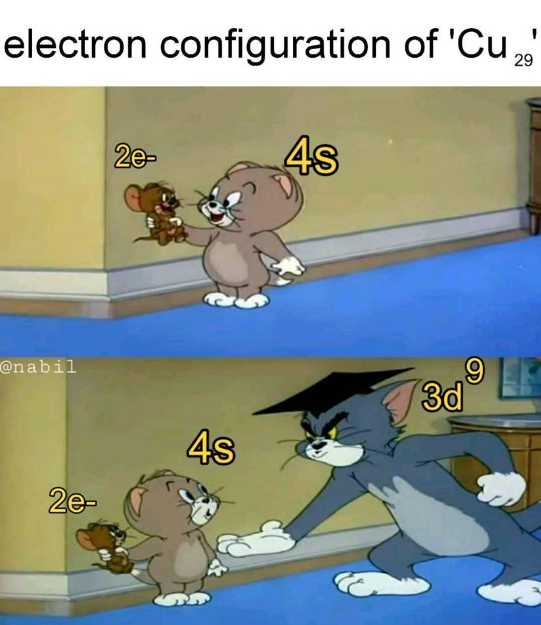
\includegraphics[trim={0 0 0 2cm}, width=0.9\textwidth, clip]{meme.png}
        \end{minipage}
\end{enumerate}

\end{document}